\documentclass[diplomskirad]{fer}

\usepackage{booktabs}
\usepackage{listings}
\usepackage[outputdir=out]{minted}

\title{Dynamic fluid visualization using smoothed particle hydrodynamics method}
\naslov{Vizualizacija dinamike fluida metodom hidrodinamike zaglađujućih čestica}
\brojrada{542}
\mentor{Krešimir Trontl}
\author{Hrvoje Hemen}
\date{June, 2024}
\datum{lipanj, 2024.}
\begin{document}
    \maketitle
    \zadatak{HrvojeHemenZadatak.pdf}
    \begin{zahvale}
        Želim se zahvaliti mentoru Krešimiru Trontlu-
    \end{zahvale}
    \mainmatter
    \tableofcontents
% TEKST RADA
    \chapter{Uvod}\label{ch:uvod}

    \section{Cilj rada}\label{sec:cilj-rada}

    Cilj ovog rada bio je napraviti realnu simulaciju dinamike fluida.
    Korištena metoda bila je metoda hidrodinamike zaglađujućih čestica (SPH).
    Inspiracija za ovaj rad bio je jedan YouTube video Sebastiana Laguea koji govori o simulaciji vode u Unityju.

    \section{Ukratko o radu}\label{sec:ukratko-o-radu}

    U sklopu ovog rada obrađeno je sve potrebno za samostalnu izradu ovog rada uključujući i postavljanje razvojnog okruženja.

    Rad je pisan u c\# programskom jeziku u sklopu Unityja, te je za vizualizaciju korišten Unityjev dvodimenzionalni vizualizator.


    \chapter{Tehnologije}\label{ch:tehnologije}

    \section{C\#}\label{sec:c}

    \begin{figure}[H]
        \centering
        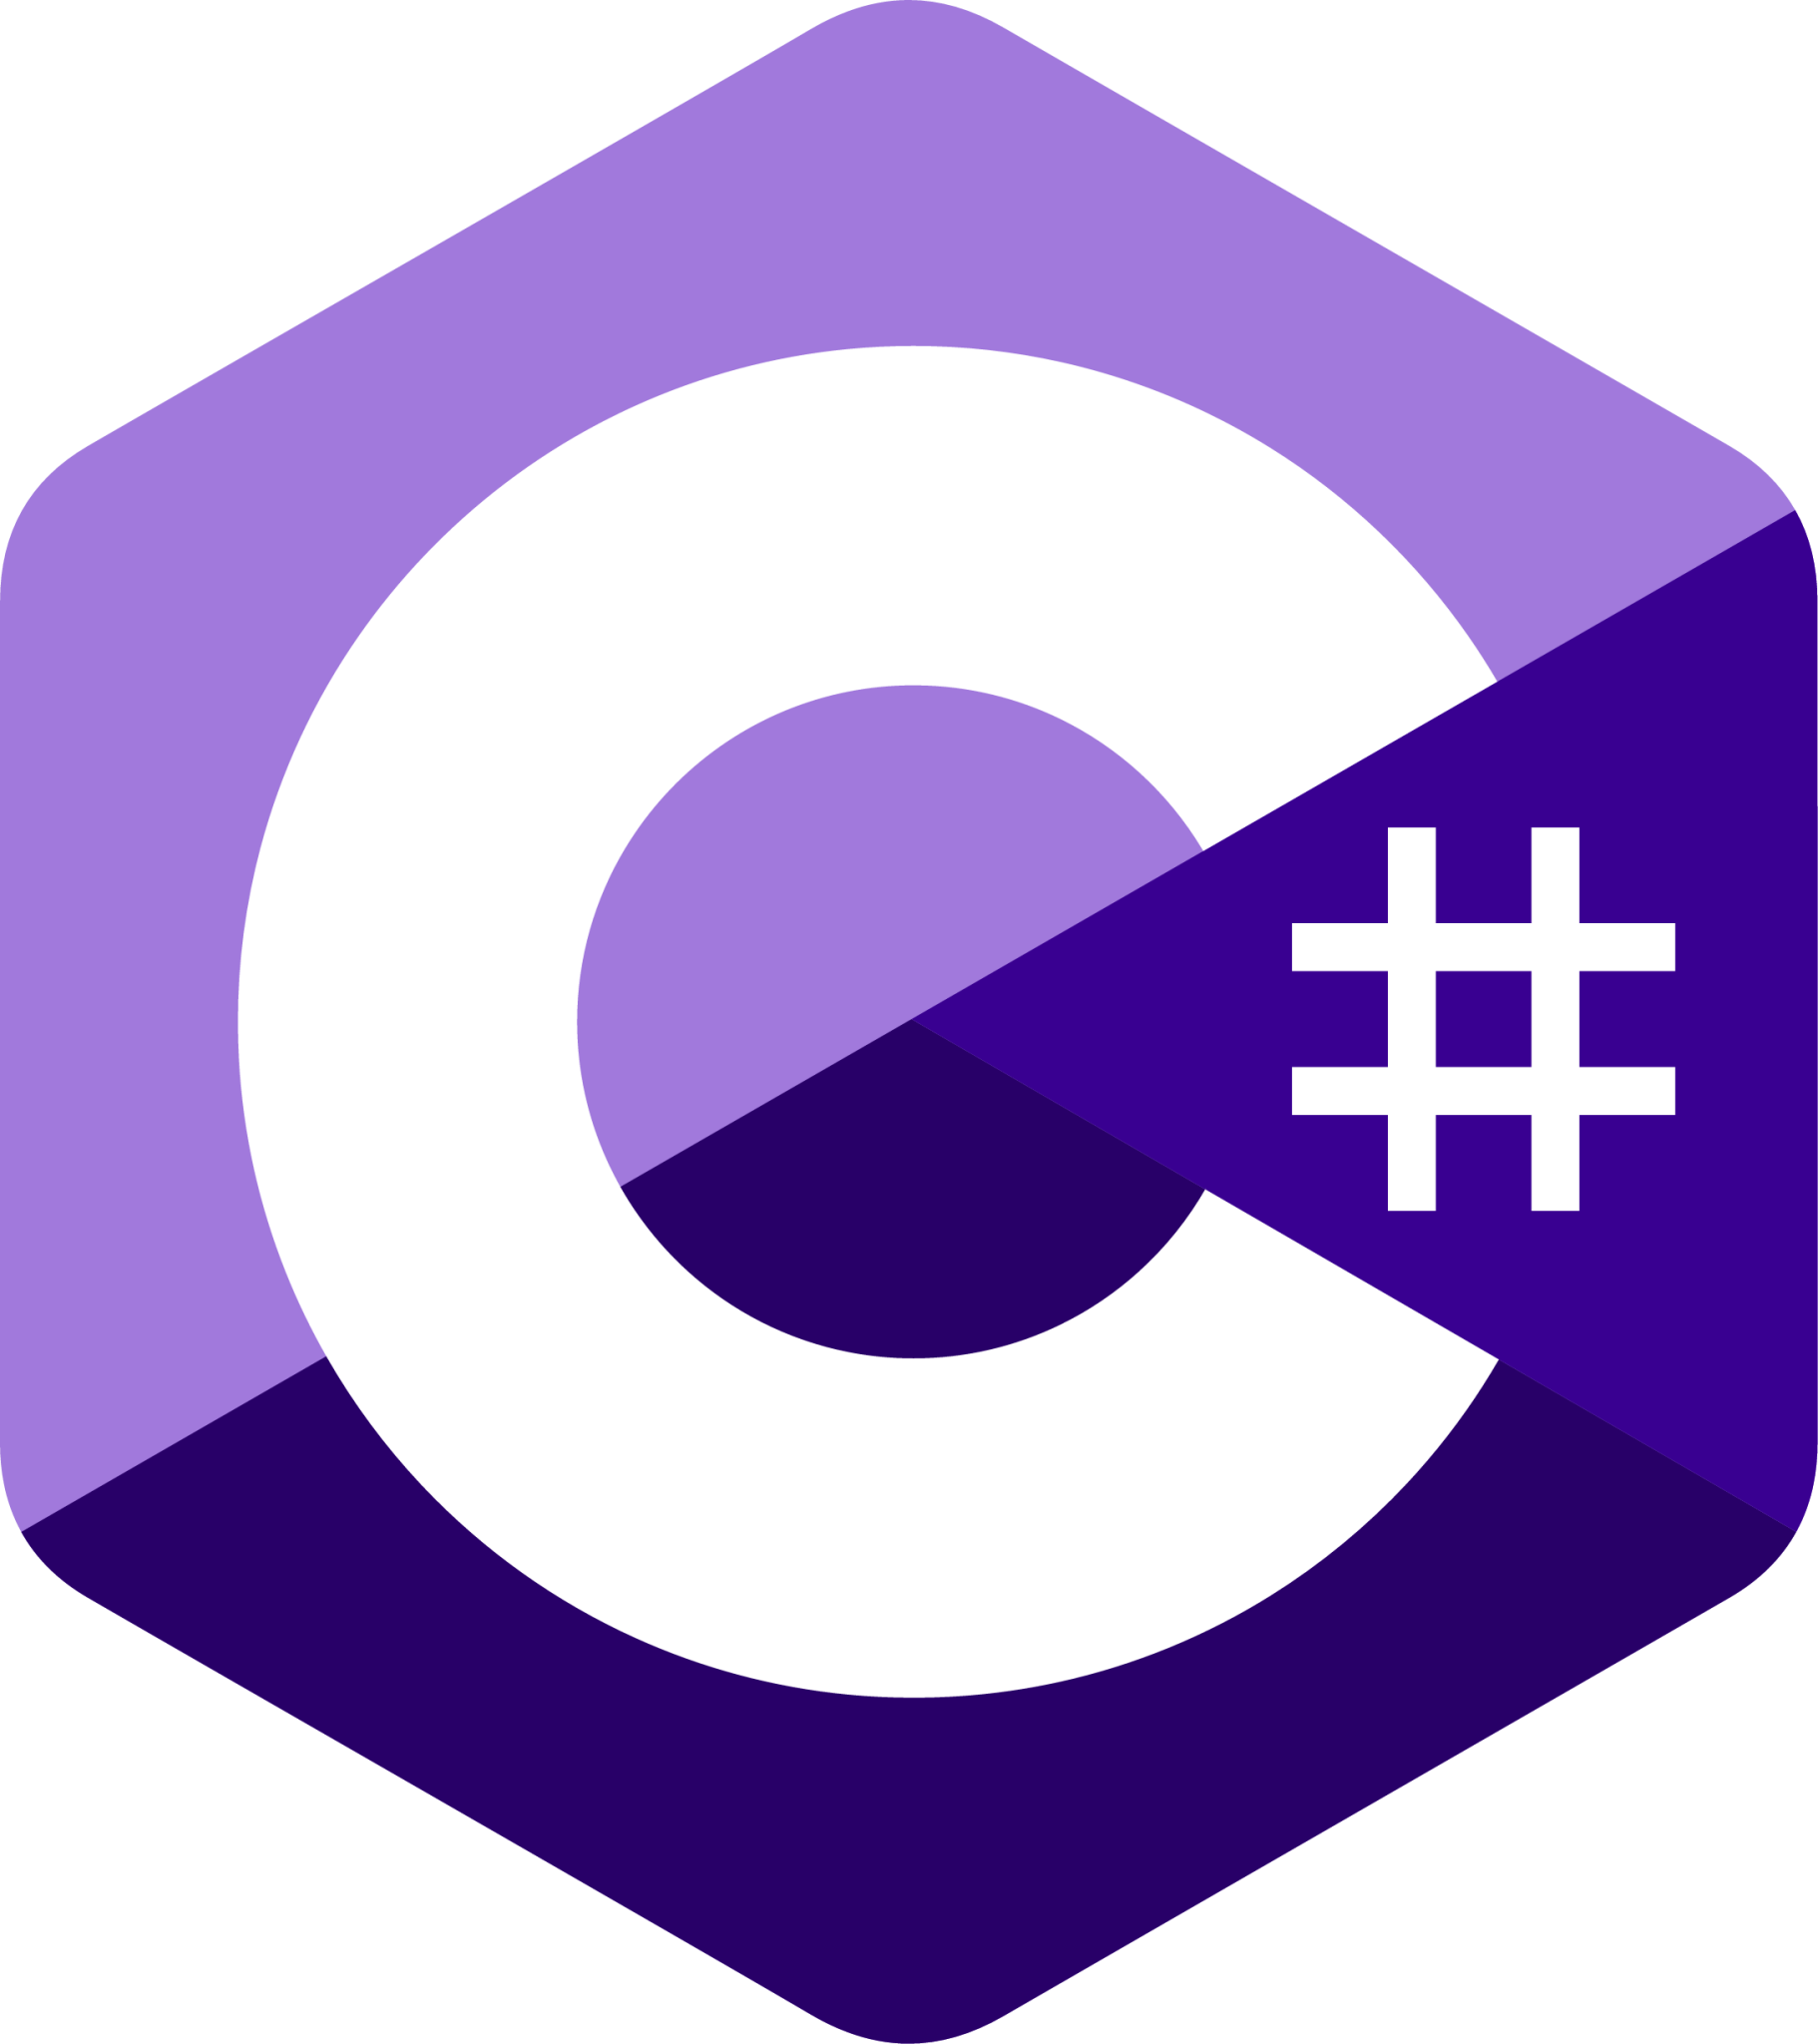
\includegraphics[scale=0.1]{images/c-sharp}
        \caption{
            C Sharp Logo \cite{cSharpLogo}
        }
        \label{fig:cSharpLogo}
    \end{figure}

    C\# je objektno orijentirani programski jezik visoke razine.
    Nastao je ranih 2000-ih zbog potrebe za objektno orijentiranim jezikom sintakse slične C jeziku.
    Najvažni ciljevi njegovog razvoja bili su jednostavnost, stroga tipiziranost,
    laka prijenosnost na različite operacijske sustave i mala potrošnja računalnih resursa.

    Sintaksa je vrlo slična Javinoj, jer svaka naredba treba završiti sa točka-zarezom \";\".
    Također, dijelovi koda omeđeni su vitičastim zagradama, koje razdvajaju kod u Klase i Metode.
    Važna razlika C\# i Jave je to što C\# omogućava preopterećenje osnovnih operacija, dakle možemo reći klasi da kada
    upotrijebimo znak plus onda radi nešto drugo, a ne matematičko dodavanje.


    \newpage
    \section{Unity}\label{sec:unity}

    \begin{figure}[H]
        \centering
        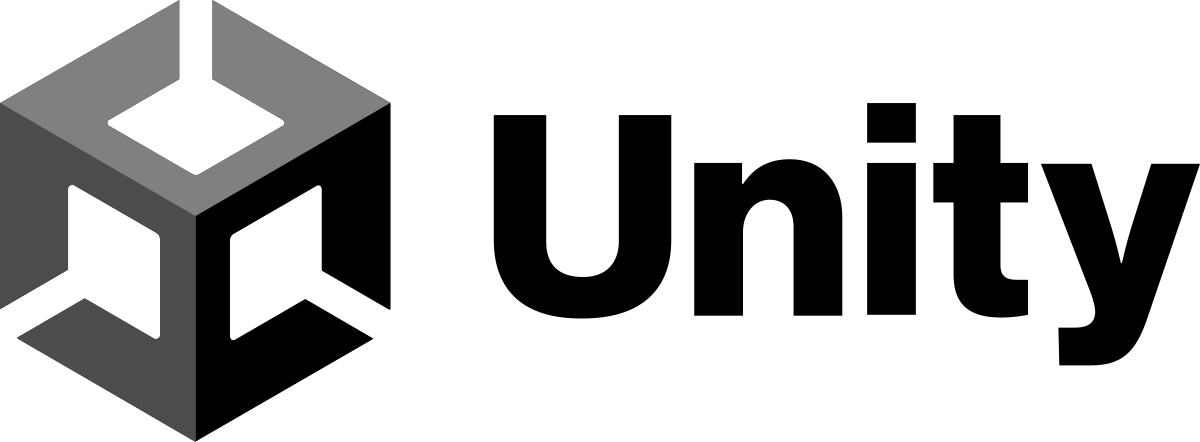
\includegraphics[scale=0.3]{images/unityLogo}
        \caption{
            Unity Logo \cite{unityLogo}
        }
        \label{fig:unityLogo}
    \end{figure}



    \chapter{Teorijska podloga}\label{ch:teorijska-podloga}

    \section{Pristupi računalnoj simulaciji fluida}\label{sec:pristupi-racunalnoj-simulaciji-fluida}

    \section{SPH metoda}\label{sec:sph-metoda}


    \chapter{Programska implementacija}\label{ch:programska-implementacija}

    \section{Osnove Unity okruženja}\label{sec:osnove-unity-okruzenja}
    \section{Osnove Unity fizičkog simulatora}\label{sec:osnove-unity-fizickog-simulatora}
    \section{čestica}\label{sec:cestica}
    \section{gustoća}\label{sec:gustoca}
    \section{pritisak}\label{sec:pritisak}
    \section{viskoza}\label{sec:viskoza}
    \section{rezultantna sila}\label{sec:rezultantna-sila}


    \bibliography{literatura}
    \begin{sazetak}
        sažetak na hrvatskom
    \end{sazetak}
    \begin{kljucnerijeci}
        ključne riječi na hrvatskom
    \end{kljucnerijeci}
    \begin{abstract}
        abstract in English
    \end{abstract}
    \begin{keywords}
        keywords in English
    \end{keywords}
\end{document}